\documentclass{article}

% Language setting
% Replace `english' with e.g. `spanish' to change the document language
\usepackage[english]{babel}

% Set page size and margins
% Replace `letterpaper' with `a4paper' for UK/EU standard size
\usepackage[letterpaper,top=2cm,bottom=2cm,left=3cm,right=3cm,marginparwidth=1.75cm]{geometry}

% Useful packages
\usepackage{amsmath}
\usepackage{graphicx}
\usepackage[colorlinks=true, allcolors=blue]{hyperref}
\usepackage{listings}
\lstset{language=R,
    basicstyle=\small\ttfamily,
    stringstyle=\color{DarkGreen},
    deletekeywords={I, df, aov},
    keywordstyle=\color{blue},
    commentstyle=\color{DarkGreen},
    numbersep=8pt
}
\usepackage{enumitem}
\renewcommand\thesubsection{\Alph{subsection}}
\usepackage{caption}
\usepackage{subcaption}
\usepackage{float}


\title{Report 1}
\author{You}

\begin{document}
\maketitle

\begin{abstract}
Your abstract.
\end{abstract}

\section{Ice cream}


\section{Hemoglobin in trout}

\begin{figure}[h]
    \centering
    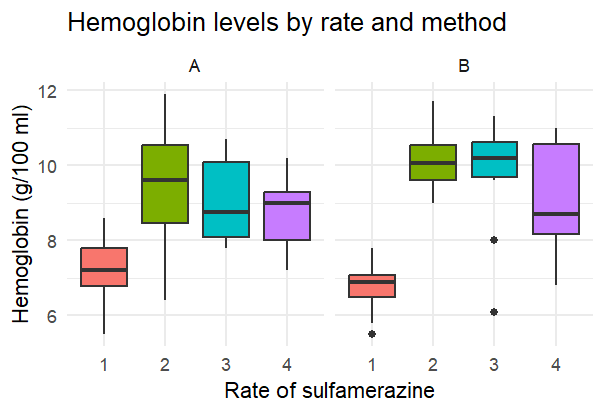
\includegraphics[height=5cm]{BoxplotHemoglobin.png}
    \caption{This boxplot illustrates the variation of hemoglobin levels across different rates of sulfamerazine, categorized by two different methods (A and B). Rates are defined as 0, 5, 10 and 15 grams of sulfamerazine per 100 pounds of fish. The rate of 1, indicating no sulfamerazine, is associated with lower hemoglobin levels compared to higher rates. }
    \label{fig:boxHem}
\end{figure}

\subsection{Randomization in R}
This dataset has an numerical data for hemoglobin and two factors (rate and method) that have levels (1,2,3,4 for rate, A and B for method). This dataset has a balanced design, because every combination of rate and method has 10 observations (N). This can be denoted as $n_{i,j} = N$, for subgroups rate (i) and method (j).
\begin{lstlisting}[caption="Randomization in R",label={lst:R}]
    rbind(rep(1:I, each = N * J), rep(1:J, N*I), sample(1:(N*I*J)))
\end{lstlisting}
in Listing \ref{lst:R}, an R-code for the randomization process to distribute 80 fishes over all combinations of levels of factors rate and method is shown.

\subsection{Two-way ANOVA}

\begin{figure}[h]
    \centering
    \begin{subfigure}{.45\textwidth}
        \centering
        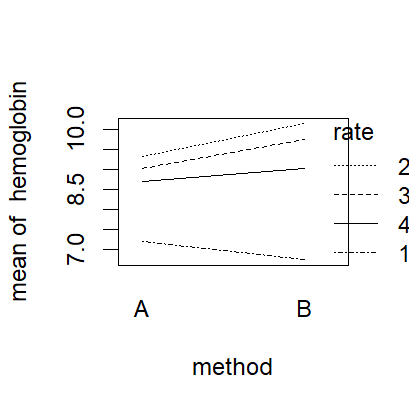
\includegraphics[height=5cm]{int_meth.png}
        \label{fig:int_rate}
    \end{subfigure}
    \begin{subfigure}{.45\textwidth}
        \centering
        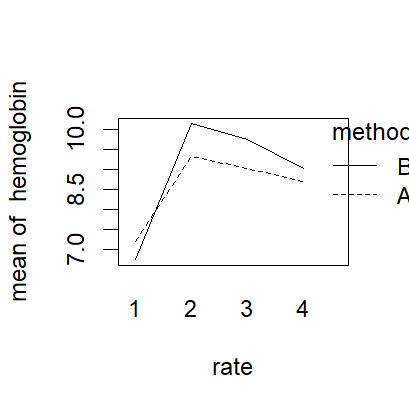
\includegraphics[height=5cm]{int_r.png}
        \label{fig:int_method}
    \end{subfigure}
    \caption{Interaction plots comparing rate and method with hemoglobin levels. }
\end{figure}

To test the effects of factors rate, method and their interaction on the response variable hemoglobin, a Two-way ANOVA test was performed following the R-code in Listing \ref{lst:T}. 
\begin{lstlisting}[caption="Two-way ANOVA", label={lst:T}]
    hemoglobin_df$rate <- as.factor(hemoglobin_df$rate) 
    hemoglobin_df$method <- as.factor(hemoglobin_df$method)
    hemoglobin_aov <- lm(hemoglobin ~ rate*method, data = hemoglobin_df)
    anova(hemoglobin_aov)   
\end{lstlisting}
rate * method indicates rate + method + rate:method, so in this test, we test if interaction can be disregarded. 

\begin{table}[ht]
\centering
\caption{Two-way ANOVA Table for Hemoglobin Levels by Rate and Method} 
\label{tab:hemoglobin_anova}
\begin{tabular}{lrrrrr}
  \hline
 & Df & Sum Sq & Mean Sq & F value & Pr($>$F) \\ 
  \hline
rate & 3 & 90.56 & 30.19 & 19.47 & 2.404e-09 \\ 
  method & 1 & 2.42 & 2.42 & 1.56 & 0.2161 \\ 
  rate:method & 3 & 4.87 & 1.62 & 1.05 & 0.3769 \\ 
  Residuals & 72 & 111.64 & 1.55 &  &  \\ 
   \hline
\end{tabular}
\end{table}

The p value for testing H0: $\gamma_{i*j}$ = 0 for all (i, j) is 0.3769. which means there is no evidence for interaction. We do not reject the hypothesis, so we can use the additive model to test which factor has most effect on the hemoglobin levels. 

\begin{table}[ht]
\caption{Treatment Parameterization in ANOVA}
\label{tab:treatment}
\centering
\begin{tabular}{rrrrr}
  \hline
 & Estimate & Std. Error & t value & Pr($>$$|$t$|$) \\ 
  \hline
(Intercept) & 7.2000 & 0.3938 & 18.28 & 0.0000 \\ 
  rate2 & 2.1300 & 0.5569 & 3.82 & 0.0003 \\ 
  rate3 & 1.8300 & 0.5569 & 3.29 & 0.0016 \\ 
  rate4 & 1.4900 & 0.5569 & 2.68 & 0.0092 \\ 
  methodB & -0.4500 & 0.5569 & -0.81 & 0.4217 \\ 
  rate2:methodB & 1.2600 & 0.7875 & 1.60 & 0.1140 \\ 
  rate3:methodB & 1.1500 & 0.7875 & 1.46 & 0.1486 \\ 
  rate4:methodB & 0.7800 & 0.7875 & 0.99 & 0.3253 \\ 
   \hline
\end{tabular}
\end{table}

Concluding from the summary of interaction ANOVA of the Hemoglobin data set in Table \ref{tab:treatment}, the combination of rate 2 with method B yields the highest hemoglobin level. The mean hemoglobin value for rate 3 by using method A can be derived from the Table \ref{tab:treatment}, is 7.200 + 1.83 = 9.03. The mean hemoglobin value for rate 2 by using method B is 7.200 + 2.13 - 0.45 + 1.26 = 10.14.

\subsection{Additive model}
\begin{lstlisting}[caption="Additive model for Two-Way ANOVA", label={lst:Add}]
    hemoglobin_aov_2 <- lm(hemoglobin ~ rate+method, data = hemoglobin_df)
    anova(hemoglobin_aov_2) 
\end{lstlisting}

\begin{table}[ht]
\caption{Additive model for Two-way ANOVA}
\label{tab:add}
\centering
\begin{tabular}{lrrrrr}
  \hline
 & Df & Sum Sq & Mean Sq & F value & Pr($>$F) \\ 
  \hline
rate & 3 & 90.56 & 30.19 & 19.43 & 2.02e-09 \\ 
  method & 1 & 2.42 & 2.42 & 1.55 & 0.2163 \\ 
  Residuals & 75 & 116.51 & 1.55 &  &  \\ 
   \hline
\end{tabular}
\end{table}

The p value for testing HA: $\alpha_i = 0$ for all i is 2.02e-09.
The p value for testing HB: $\beta_j = 0$ for all j is 0.2163.
So only rate of sulfamerazine has a main effect in the additive model.

\begin{table}[ht]
\caption{Treatment Parameterization for additive model}
\label{tab:treatment_add}
\centering
\begin{tabular}{rrrrr}
  \hline
 & Estimate & Std. Error & t value & Pr($>$$|$t$|$) \\ 
  \hline
(Intercept) & 6.8012 & 0.3116 & 21.83 & 0.0000 \\ 
  rate2 & 2.7600 & 0.3941 & 7.00 & 9.18e-10 \\ 
  rate3 & 2.4050 & 0.3941 & 6.10 & 4.24e-08 \\ 
  rate4 & 1.8800 & 0.3941 & 4.77 & 8.86e-06 \\ 
  methodB & 0.3475 & 0.2787 & 1.25 & 0.2163 \\ 
   \hline
\end{tabular}
\end{table}

\subsection{One-way ANOVA}
Because we did not observe any effect of the factor method, it may provide useful to ignore the variable method and perform a One-Way ANOVA for all rates. 
\begin{lstlisting}[caption="One-Way ANOVA", label={lst:owa}]
    rate_aov <- lm(hemoglobin ~ rate, data = hemoglobin_df)
    anova(rate_aov)
\end{lstlisting}
Testing H0: $\alpha_1=...=\alpha_4$ is rejected with a p value of 2.129e-09.
The rate of sulfamerazine seems to have a significant effect on the hemoglobin level
Is it useful?

\subsection{Kruskal-Wallis test}
\begin{lstlisting}[caption="Kruskal-Wallis", label={lst:kw}]
    kruskal.test(hemoglobin ~ rate, data = hemoglobin_df)
\end{lstlisting}
The p-value for this test is 1.777e-07

\begin{figure}[h]
    \centering
    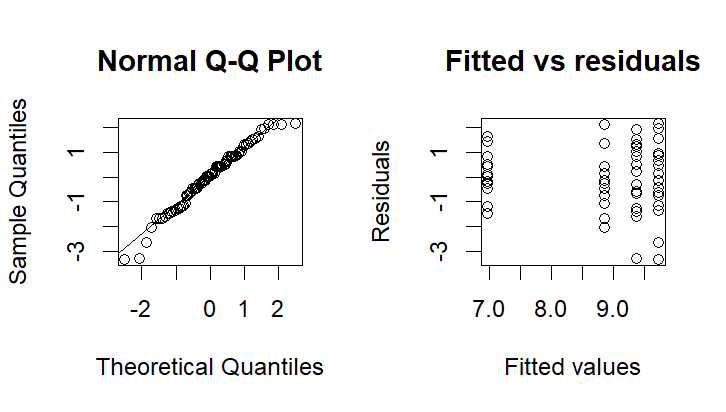
\includegraphics[height=5cm]{normal_fit_res_ex2.png}
    \caption{The left graph shows qqnorm plot of the residuals and the right plot the fitted values against residuals.}
    \label{fig:norfitresex2}
\end{figure}
When applying any ANOVA model to a dataset, it is important to check normality of errors. This can be done by the two following tools: qqnorm plot of the residuals and the plot of fitted against residuals, which are visualized in Figure \ref{fig:norfitresex2}.  
The residuals do not seem to deviate significantly from
normal and the plot of the fitted values $Y_ik = \mu_i$ against
the residuals $e_ik$ does not show a pattern, which means both ANOVA and Kruskal-Wallis could be used here. Whenever the normality assumption fails, only the Kruskal-Wallis test could be used, as it does not rely on normality and is based on ranks. 

\section{Exercise 3}

\subsection{Difference in acidity Starter 1 \& Starter 2.}

\begin{table}[H]
\centering
\begin{tabular}{lcccc}
\hline
\textbf{Predictor} & \textbf{Estimate} & \textbf{Std. Error} & \textbf{t value} & \textbf{Pr$(>|t|)$} \\
\hline
(Intercept) & 8.6616 & 0.5329 & 16.255 & $<$0.0001\\
starter2    & -0.1500 & 0.4673 & -0.321 & 0.7538    \\
starter3    & -0.9800 & 0.4673 & -2.097 & 0.0579  \\
starter4    & 2.8100 & 0.4673 & 6.013  & $<$0.0001\\
starter5    & -0.4840 & 0.4673 & -1.036 & 0.3208    \\
batch2      & -1.3480 & 0.4673 & -2.884 & 0.0137  \\
batch3      & 0.2760 & 0.4673 & 0.591  & 0.5658    \\
batch4      & 1.3680 & 0.4673 & 2.927  & 0.0127  \\
batch5      & 0.2000 & 0.4673 & 0.428  & 0.6763    \\
position2   & -0.6180 & 0.4673 & -1.322 & 0.2107    \\
position3   & -0.0380 & 0.4673 & -0.081 & 0.9365    \\
position4   & -0.7640 & 0.4673 & -1.635 & 0.1280    \\
position5   & -0.2640 & 0.4673 & -0.565 & 0.5825    \\
\hline
\end{tabular}
\caption{Summary of linear model for acidity.}
\label{table:acidity}
\end{table}

Table \ref{table:acidity} shows the estimates for starter2, starter3, starter4, and starter5 and how they differ in acidity on average compared to the reference category starter1. the same goes for batch and position and how they differ from their reference batch1 and position1. 

To see if there is a significant difference between starter1 and starter2 we have to account for 2 main values, the estimate and the p-value. We can see that the estimate from starter2 doesn't differ much from starter1, especially when we compare it to starter4. Considering the p-value for starter2 (0.7538) which is very high, 0.05 is supposed to signify high significance



\subsection{B}



\subsection{C}

\subsection{D}


\bibliographystyle{alpha}
\bibliography{sample}

\end{document}